
\section*{Ejercicios}
\addcontentsline{toc}{section}{\textit{Ejercicios}}

\begin{Enunciado}
\subsection*{Ejercicio 1}


	Se dopa silicio con Boro (B) en una proporción de 2 ppm (partes por millón)
	\begin{enumerate}[label=\alph*)]
		\item Calcula la concentración intrínseca del Si y obten una expresión de dicha concentración en función de la temperatura.
		\item Indica el tipo de conducción de este material y calcula la concentración de impurezas y la de electrones y huecos (n y p) a temperatura ambiente si todos los dopantes están ionizados.
		\item Calcula la posición del nivel de Fermi y dibuja el diagrama de bandas completo correspondiente.
		\item ¿Qué pasa si la concentración de impurezas igualase el valor de \( N_V \)? Representa gráficamente las bandas de energía frente a la concentración de impurezas usando todas las aproximaciones que conozcas.
	\end{enumerate}
	(DATO: Constante de red del Si \( a_0 = 5.431 \) Å).

\end{Enunciado}

	Veamos las soluciones por apartados
	\begin{enumerate}[label=\alph*)]
		\item La concentración intrínseca del Silicio en un semiconductor es el número de portadores $n_i$ en el semiconductor, si no estuviera dopado. No hay que confundir la concentración intrínseca $n_i$ con la concentración $n$, en la que si se tendrá en cuenta que el material está dopado. La concentración intrínseca es:

		      \begin{equation}
			      n_i = \sqrt{N_cN_v} e^{-E_G/2kT}
		      \end{equation}
		      donde $E_G=E_c-E-v$, y además

		      \begin{equation}
			      N_{C,V} = 2 \parentesis{\frac{m_{e,p}^* kT}{2\pi\hbar^2}}^{-3/2}
		      \end{equation}
		      Las masass $m_p^*= 1.18m_e$ y $m_n^*=0.81m_e$. Si queremos dar el valor:

		      \begin{equation}
			      N_c = 3.22 \cdot 10^{19} \cm^{-3} \tquad 	N_v = 1.83 \cdot 10^{19} \cm^{-3}
		      \end{equation}
		      De lo que se deduce

		      \begin{equation}
			      n_i = 9.56 \cdot 10^9 \cm^{-3}
		      \end{equation}


		\item Están dopando con boro, que es del grupo III, y por tanto es un dador. Esto significa que será un conductor tipo $p$. Para calcular la concentración de impurezas, primero tenemos que obtener la densidad de Boro en nuestro silicio. La densidad del silicio se calcular a partir de la constante de red y sabiendo que posee una red diamante. Así pues:
		      \begin{equation}
			      N_{Si} = \frac{8}{a_0^3}
		      \end{equation}
		      de lo que se puede deducir entonces que:
		      \begin{equation}
			      N_B = 2\cdot 10^{-6} \cdot N_{Si} = 9.988 \cdot 10^16 \cm^{-3}
		      \end{equation}
		      Nos dicen que todos los dopantes están ionizados, es decir, que estamos en el régimen extrínseco. En este régimen todos los átomos de Boro son impurezas, tal que $N_A^-=N_A=N_B$. Suponiendo que $N_A^- \gg N_D^+$, tenemos que la ecuación de neutralidad de carga:

		      \begin{equation}
			      n\cdot p = n_i^2 \tquad p-n-N_A = 0
		      \end{equation}
		      usando estas ecuaciones para despejar el valor de $n$ y $p$, tenemos que:
		      \begin{equation}
			      p = \frac{N_A}{2} + \ccorchetes{\parentesis{\frac{N_A}{2}}^2 + n_i^2}^{1/2}
		      \end{equation}
		      y luego calculamos

		      \begin{equation}
			      n = \frac{n_i^2}{p}
		      \end{equation}
		      Numéricamente podemos obtener los resultados:

		      \begin{equation}
			      n=915.034 \cm^{-3} \quad p = 9.988 \cdot 10^{16} \cm^3
		      \end{equation}


		\item La posición del nivel de Fermi de un semiconductor dopado se calcula a partir del nivel de Fermi intrínseco. Así pues
		      \begin{equation}
			      E_{Fi} = E_i = \frac{E_c+E_v}{2} + \frac{3 kT}{4} \ln \frac{m_p^*}{m_e^*} = 0.523 \text{eV}
		      \end{equation}
		      tal que la energía de Fermi. *Introducir imagen*
		      \begin{equation}
			      E_F = E_i + kT \ln \parentesis{\frac{p}{n_i}} = 0.135 \text{0.135}
		      \end{equation}
		\item Cuando la concentración de impurezas es igual al valor de $N_V$, dado que $p=N_V e^{(E_v-E_F)/kT}$, esto implicaría que $E_v = E_F$, y que por tanto la condición de \textit{semiconductor no degnerado} $E_F>E_v + 3kT$ no se cumpliría. \textit{Tenemos un semiconductor degenerado, teniendo que calcular los valores de $n$ y $p$ mediante las integrales explícitas}. Consecuentemente, estamos ante un semiconductor degenerado. *Introducir imagen para las bandas*.
	\end{enumerate}
\begin{Enunciado}
\subsection*{Ejercicio 2}

	Una muestra de Si está dopada con \( 6 \times 10^{15} \) átomos de As por cm$^3$
	\begin{enumerate}[label=\alph*)]
		\item ¿Cuál es la concentración de portadores en la muestra de Si a 300 K?
		\item ¿Cuál es la concentración de portadores a 470 K?
		\item Para cada una de las dos temperaturas anteriores determinar la posición de \( E_i \), calcular \( E_F - E_i \) y dibujar a escala el diagrama de bandas de energía para la muestra.
		\item Si dopamos el Si con \( 10^{16} \) átomos donadores y \( 5 \times 10^{15} \) átomos aceptores por cm$^3$. ¿Cuál es la concentración de portadores a 300 K?+
		\item Partimos de una muestra de Si puro y lo dopamos exclusivamente con \( 10^{14} \) átomos donadores y \( 10^{14} \) átomos aceptores por cm³. Calcula la concentración de portadores y explica el resultado obtenido.
	\end{enumerate}
	Tener en cuenta que \( E_G = 1.08 \) eV a 470 K y suponer que \( m_e^*/m_h^* = 0.69 \) es independiente de la temperatura.

\end{Enunciado}

	\begin{enumerate}[label=\alph*)]
		\item Tenemos primero que ver si está degenerado, sin embargo sabemos que para esta temperatura y el nivel de dopamiento no debería estar degenerado, y por tanto podríamos usar la ley de acción de masas junto con la condición de electroneutralidad para despejar $n$ en función de $N_D,N_A$ y $n_i$. Se puede obtener, dado que $N_D \gg n_i,N_A$, tenemos que

		      \begin{equation}
			      n\approx N_D = 6\cdot 10^{15} \cm^{-3} \tquad n\cdot p = n_i^2 \Rightarrow p = 1.67 \cdot 10^4 \cm^{-3}
		      \end{equation}
		\item Nos dicen que a $T=470$K y que $E_G=1.08$eV. Lo único que no cambio es $N_D$. Lógicamente el número de portadores intrínsecos $n_i$ cambia al aumentar la temperatura: a mayor energía térmica promocionan más electrones, mas electrones van a poder excitarse desde la banda de valencia. Calculamos $n_i$ a partir de
		      \begin{equation}
			      n_i = \sqrt{N_cN_v} e^{-E_g/2kT}
		      \end{equation}
		      Luego solo tenemos que hacer

		      \begin{equation}
			      N_{c,v} = 4.829\cdot 10^{15} T^{3/2} \parentesis{\frac{m_{n,p}^*}{m_e}}
		      \end{equation}
		      A esta temperatura tenemos entonces que:

		      \begin{equation}
			      N_c = 6.3 \cdot 10^{19} \cm^{-3} \quad N_v = 3.6 \cdot 10^{19} \cm^{-3}
		      \end{equation}
		      Y por tanto

		      \begin{equation}
			      n_i = 7.74 \cdot 10^{13} \cm^{-3}
		      \end{equation}
		      De lo que se deduce, de nuevo, aplicnado la ley de acción de masas:

		      \begin{equation}
			      n=6.001 \cdot 10^{15} \cm^{-3} \quad p = 9.98 \cdot 10^{11} \cm^{-3}
		      \end{equation}
		\item Determina la posción del nivel de Fermi intrínseco. Es secillo que:
		      \begin{equation}
			      E_i = \frac{E_c + E_v}{2} + \frac{3}{4} kT \ln \parentesis{\frac{m_p^*}{m_n^*}}
		      \end{equation}
		      Una vez tenemos $E_i$ para cada una de las temperaturas, calculamos la temperatura final
		      \begin{equation}
			      E_F = E_i + kT \ln \parentesis{\frac{n}{n_i}}
		      \end{equation}
		      *Introducir imagen*
		\item.
		\item
	\end{enumerate}
    
\begin{Anotacion}
    \textcolor{red}{\textbf{Falta por acabar}}
\end{Anotacion}
\begin{Enunciado}
\subsection*{Ejercicio 3}

	Cuestiones sobre el nivel de Fermi:

	\begin{enumerate}[label=\alph*)]
		\item Calcular la temperatura \( T \) para que el nivel de Fermi de un cristal de Silicio tipo N con \( N_D = 10^{16} \) cm\(^{-3}\) quedara a una energía \( E_G/3 \) por debajo de la banda de conducción. Suponer que \( N_C \) y \( E_G \) son constantes con la temperatura e iguales a sus valores a temperatura ambiente. Y repetir para el caso de dopar con \( N_D = 10^{18} \) cm\(^{-3}\).

		\item En un semiconductor determinado, la probabilidad de que los electrones ocupen un estado de energía \( kT \), por encima del extremo inferior de la banda de conducción es \( e^{-10} \). Determinar la posición del nivel de Fermi en dicho material.

		\item ¿Cuál es la probabilidad de que un estado de energía \( kT \) por debajo del nivel de Fermi esté ocupado por un hueco?
	\end{enumerate}

\end{Enunciado}

	\begin{enumerate}[label=\alph*)]
		\item La solución es $T=536.206$K. Para esto tenemos que usar la relación
		      \begin{equation}
			      T = \frac{E_F-E_c}{k} \frac{1}{\ln (N_D/N_c)} =  \frac{-E_g}{3k} \frac{1}{\ln (N_D/N_c)}
		      \end{equation}
		      donde $N_c=3.22\cdot 10^{19}\cm^{-3}$.
		\item Queremos calcular la posición del nivel de Fermi. Usamos la fórmula
		      \begin{equation}
			      f(E) = \frac{1}{1+e^{(E-E_F)/kT}}
		      \end{equation}
		      y usando lo que nos da el enunciado:
		      \begin{equation}
			      f(kT+E_c) = \frac{1}{1+e^{(kT+E_c-E_F)/kT}}
			      = \frac{1}{e^{10}}
		      \end{equation}
		      Tenemos entonces que

		      \begin{equation}
			      1+e^{\frac{kT+E_c-E_f}{kT}} = e^{10}
		      \end{equation}
		      De lo que se deduce que $E_F = E_c + 9kT$.
		\item ¿Cuál es la probabilidad de que un estado de energía \( kT \) por debajo del nivel de Fermi esté ocupado por un hueco? Tenemos que
		      \begin{equation}
			      1-f(E_F-kT) = 1 - \frac{1}{1+e^{-1}} \simeq 0.2689 \rightarrow 26.89 \%
		      \end{equation}
		      La probabilidad es no nula y por tanto... (preguntar a Elisa Casal).
	\end{enumerate}

\begin{Enunciado}
\subsection*{Ejercicio 4}

Responde a las siguientes cuestiones:
\begin{enumerate}
	\item[a)] A 300 K la densidad efectiva de estados en la banda de valencia es $1.83 \times 10^{19} \text{ cm}^{-3}$ para el silicio y $9.0 \times 10^{18} \text{ cm}^{-3}$ para el GaAs. Calcular sus correspondientes masas efectivas para los huecos. Comparar estas masas con la masa del electrón en el vacío.

	\item[b)] Calcula y representa la posición del nivel intrínseco en silicio a temperatura ambiente y a 1000 $^{\circ}$C (tomamos $m_p = 1.0m_0$ y $m_n = 0.19m_0$), asumiendo que el gap se mantiene constante. ¿Es razonable asumir que $E_i$ se encuentra en la mitad de la banda prohibida?
\end{enumerate}
\end{Enunciado}

\begin{enumerate}[label=\alph*)]
	\item	Tenemos que calcular la masa efectiva de los huecos para dos semiconductores diferentes, dado su densidad efectiva de estados en la banda de valencia. Esto significa que necesitamos invertir la fórmula típica, tal que
		  \begin{equation}
			  N_V = 2 \parentesis{\frac{m_p^* kT}{2\pi\hbar^2}}^{3/2} \quad \Rightarrow \quad m_p^* = \parentesis{\frac{N_V}{2}}^{2/3} {\frac{2 \pi \hbar^2}{kT}}
		  \end{equation}
		  De lo que se deduce que para el Si y el GsAs:

		  \begin{equation}
			  \text{Si:} \quad m_p^* = 7.38\cdot10^{-31} \text{kg} = 0.81 \ {m}_e
		  \end{equation}
		  \begin{equation}
			  \text{GaSi:}\quad m_p^* = 4.59 \cdot10^{-31} \text{kg} = 0.51 \ {m}_e
		  \end{equation}
		  Nivel intríseco 300K 1.7505319217070854
	\item Tenemos que calcular la posición del nivel intrínseco $E_i$ a la temperatura ambiente (300 K) y a 1000 $^\circ C$, asumiendo que $E_g$ es constante. Veamos que solo es aplicar una fórmula:
		  \begin{equation}
			  E_i = \frac{E_c+E_v}{2} + \frac{3}{4} kT \ln\parentesis{\frac{m_p^*}{m_n^*}}
		  \end{equation}
		  donde hemos considerado que $E_g=1.12$ en el silicio, y que $E_v=0$, ergo $E_c=1.12$. Hacemos la representación gráficamente. Las energías son: $300K: \ E_i=0.57$ eV y a 1273K $E_i: 0.70$ eV. Las masas usadas a 300K son: $m_p=0.81m_e$ y $m_n=1.18m_e$.
		  \begin{center}
			  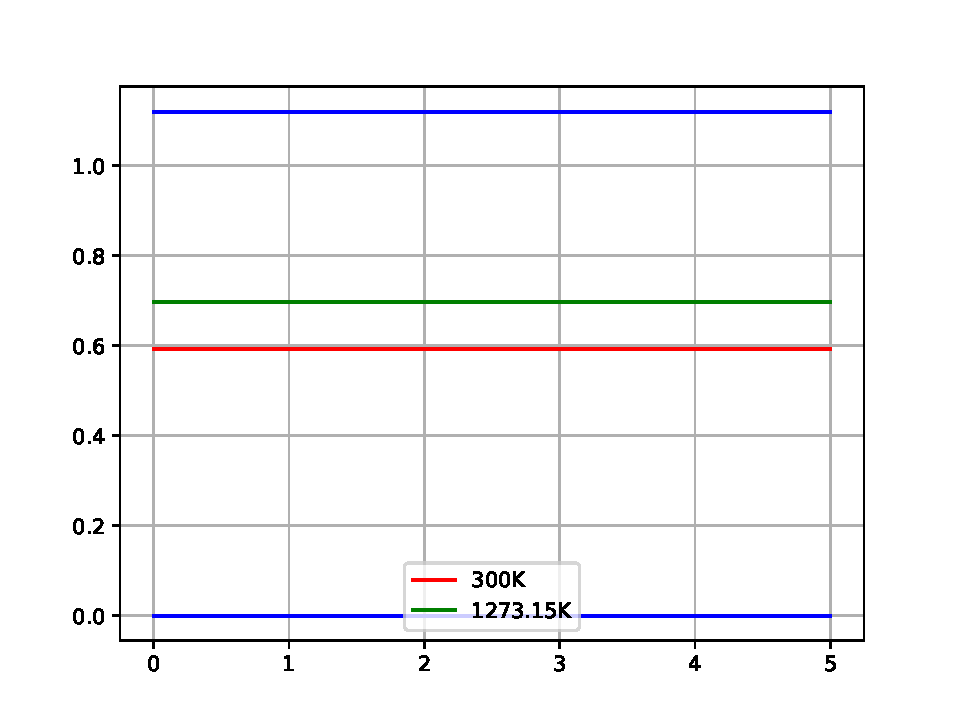
\includegraphics[width=0.6\textwidth]{Ejercicios/Ch_01/Ejercicio_01_5.pdf}
		  \end{center}
		  Viendo esta imagén no parece descabellado consdierar $E_i$ constante.
\end{enumerate}


\begin{Enunciado}
	
\subsection*{Ejercicio 5}

\begin{enumerate}[label=\alph*)]
	\item En GaN a 300 K, $E_G = 3.43$ eV, $m_n^*/m_0 = 0.2$, $m_p^*/m_0 = 1.25$ y $n_i = 1.37 \times 10^{-10} \text{ cm}^{-3}$. Explicar cualitativamente (sin utilizar la fórmula que calcula el valor de $E_i$) si el nivel de Fermi intrínseco en InSb estará más próximo a la $E_C$ o a la $E_V$. Comprobarlo a continuación usando la fórmula.

	\item Las distribuciones de portadores, o número de portadores en función de la energía en las bandas de conducción y de valencia presentan un máximo a una energía próxima a los bordes de las bandas. Considerando el semiconductor como no degenerado, calcular la energía a la que se encuentra el máximo en la distribución de electrones.
\end{enumerate}
\end{Enunciado}


\begin{enumerate}[label=\alph*)]
	\item El nivel de Fermi intrínseco a temperatura no nula está mas cerca de $E_c$ si la masa efectiva de los huecos es mayor que la masa efectiva de los electrones, y más cerca de $E_v$ si la masa de los electrones es mas grande que la de los huecos. ¿Por qué? Como sabemos, la masa efectiva de los electrones/huecos es inversamente proporcional a la curvatura en el mínimo/máximo de la banda de conducción/valencia. Cuanto mayor sea la curvatura, mas energía se tiene que darse para ocupar la misma cantidad de estados. Como consecuencia, la energía de fermi intríseca, que se define como la mitad del valor entre $E_c$ y $E_v$ tendría que tirar hacia la banda con más curvatura, i.e. la que tiene menos masa efectiva. \textcolor{BrickRed}{Francamente no me tiene mucho sentido, ya que $E_c$ y $E_v$ no debería cambiar. Existen otras formas de verlo a través de la función de Fermi y la densidad de estados, habría que investigarlo.}

	En nuestro caso esto implica que \textit{debería estár mas cerca de la banda de conducción}. Para los valores dados, tenemos que

	\begin{equation}
		  E_i = \frac{E_c+E_v}{2} + \frac{3}{4} kT \ln\parentesis{\frac{m_p^*}{m_n^*}} = 1.75 \ \text{eV}
	\end{equation}
	que considerando $E_v=0$ y $E_c=E_g=3.43$ eV vemos que está mas cerca de la banda de conducción $E_c$ que de $E_v$.
	\item La concentración de electrones en la banda de conducción está dada por:

		  \[
			  n(E) = g_c(E) f(E)
		  \]

		  donde

		  \begin{itemize}
			  \item La densidad de estados en la banda de conducción es:

					\[
						g_c(E) = \frac{8\pi \sqrt{2} m_c^{3/2}}{h^3} (E - E_c)^{1/2}
					\]

			  \item La función de distribución de Fermi-Dirac en la aproximación no degenerada (Maxwell-Boltzmann) es:

					\[
						f(E) \approx e^{-\frac{(E - E_F)}{k_B T}}
					\]
		  \end{itemize}

		  Por lo que la distribución de portadores en la banda de conducción es:

		  \[
			  n(E) = \frac{8\pi \sqrt{2} m_c^{3/2}}{h^3} (E - E_c)^{1/2} e^{-\frac{(E - E_F)}{k_B T}}
		  \]

		  Para encontrar el máximo, derivamos respecto a \( E \) e igualamos a cero:

		  \[
			  \frac{d}{dE} \left[ (E - E_c)^{1/2} e^{-\frac{(E - E_F)}{k_B T}} \right] = 0
		  \]

		  Aplicando la regla del producto:

		  \[
			  \frac{1}{2} (E - E_c)^{-1/2} e^{-\frac{(E - E_F)}{k_B T}} + (E - E_c)^{1/2} e^{-\frac{(E - E_F)}{k_B T}} \left(-\frac{1}{k_B T} \right) = 0
		  \]

		  Factorizando:

		  \[
			  e^{-\frac{(E - E_F)}{k_B T}} (E - E_c)^{-1/2} \left[ \frac{1}{2} - \frac{(E - E_c)}{k_B T} \right] = 0
		  \]

		  Para que se cumpla la igualdad, la expresión entre corchetes debe ser cero:

		  \[
			  \frac{1}{2} = \frac{(E - E_c)}{k_B T}
		  \]

		  Despejando \( E \):

		  \[
			  E - E_c = \frac{1}{2} k_B T
		  \]
		  Por lo tanto, el máximo de la distribución de electrones en la banda de conducción se encuentra a:

		  \[
			  E_{\text{max}, c} = E_c + \frac{1}{2} k_B T
		  \]

		  Siguiendo el mismo procedimiento para los huecos en la banda de valencia:

		  \[
			  E_{\text{max}, v} = E_v - \frac{1}{2} k_B T
		  \]

		  Esto significa que los portadores tienden a concentrarse en energías lige,amente por encima del borde de la banda de conducción y por debajo del borde de la banda de valencia en aproximadamente \( \frac{1}{2} k_B T \). El doctorando hizo un dibujo que dijo que sale en el Pierret, sobre la multiplicación de producto de la densidad de estados y las bandas. Véase notas a mano.

\end{enumerate}


\begin{Enunciado}
\subsection*{Ejercicio 6}

Dibujar un diagrama de bandas para el silicio dopado con $10^{17}$ átomos/cm$^3$ de arsénico a 300 K y 600 K. Mostrar el nivel de Fermi, $E_C$, $E_V$ y utilizar el nivel de Fermi intrínseco como energía de referencia, asumiendo el caso de ionización total. La variación del bandgap con la temperatura viene dada por la expresión de Varshni (DOI: 10.1016/0031-8914(67)90062-6):

\begin{equation}
	E_G(T) = E_G(0) - \frac{\alpha T^2}{T + \beta}
\end{equation}

Para el silicio $\alpha = 4.73 \times 10^{-4} \text{ eV/K}$, $\beta = 636 \text{ K}$ y $E_G(0) = 1.17 \text{ eV}$. Suponer que las masas efectivas se mantienen constantes con la temperatura.

\end{Enunciado}


Nos dicen que dibujemos un diagrama de bandas para el silicio dopado por arsénico (grupo V, dador) completamente ionizado. Esto implica necesariamente calcular $E_i,E_c,E_v$ y $E_F$. Primero vamos a despejar $E_i$ y $E_v$, luego despejaremos en función de estos $E_F$. Recordar que

\begin{equation}
	E_i = \frac{E_v+E_c}{2} - \frac{3}{4} kT \ln\parentesis{\frac{m_n^*}{m_p^*}}
\end{equation}

\begin{itemize}
	\item Como hemos dicho despejamos estas energías. Dado que $E_i$ es nuestra referencia, las ecuaciones a usar son, a una $T$ dada, que:
		  \begin{equation}
			  E_c-E_v = E_g(0) - \frac{\alpha T^2}{T+\beta} \qquad E_c+E_v=-2 \cdot \frac{3}{4} kT\ln \parentesis{\frac{m_n^*}{m_p^*}}
		  \end{equation}
		  De lo cual se deduce que:
		  \begin{equation}
			  E_c = \frac{1}{2} \ccorchetes{E_g(0) - \frac{\alpha T^2}{T+\beta} - \frac{3}{2} kT^{3/2} \ln \parentesis{\frac{m_n^*}{m_p^*}}}
		  \end{equation}
		  \begin{equation}
			  E_v = \frac{1}{2} \ccorchetes{-E_g(0) +\frac{\alpha T^2}{T+\beta} - \frac{3}{2} kT^{3/2} \ln \parentesis{\frac{m_n^*}{m_p^*}}}
		  \end{equation}
		  Usando las masas de portadores $m_n^*=1.18m_e$ y $m_p^*=0.81m_e$  (y considerado, como nos dice el enunciado, que son constantes frente a la tempratura). Obteniendo los siguientes resultados numéricos:
		  \begin{equation}
			  \text{300K}: \qquad
			  E_c = 0.570 \ \text{eV} \quad E_v = -0.554 \ \text{eV}
		  \end{equation}
		  \begin{equation}
			  \text{600K}: \qquad
			  E_c = 0.531  \ \text{eV} \quad E_v = -0.502\ \text{eV}
		  \end{equation}
	\item Ahora tenemos que calcular $E_F$, que viene dado, en un conductor dopado $N$ no degnerado por (recordar que $E_i=0$)
		  \begin{equation}
			  E_F = kT \ln \parentesis{\frac{N_D}{n_i}}
		  \end{equation}
		  Dado que conocemos $T$ y $N_D$, solo resta saber el valor de $n_i$, para lo cual hemos usado la expresión:

		  \begin{equation}
			  n_i = \sqrt{N_c N_v} e^{-E_g/2kT}
		  \end{equation}
		  siendo $N_c$ y $N_v$ las típicas funciones que dependen de la masa efectiva y del a temperatura. Así pues, obtenemo los resultados:
		  \begin{equation}
			  \text{300K:}\quad
			  E_F = 0.420 \ \text{eV} \qquad
			  \text{600K:}\quad
			  E_F= 0.178 \ \text{eV}
		  \end{equation}
\end{itemize}
Una vez tenemos esto podemos realizar la representación:
\begin{center}
	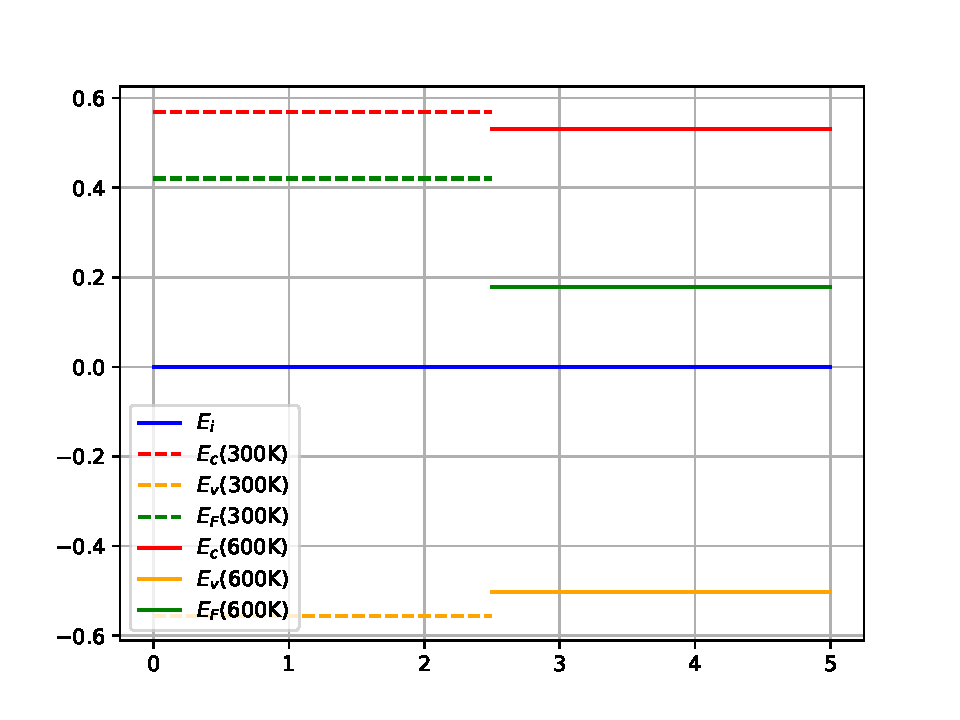
\includegraphics[width=0.9\linewidth]{Ejercicios/Ch_01/Ejercicio_01_7.pdf}
\end{center}


\begin{Enunciado}
\subsection*{Ejercicio 7}
Calcular el nivel de Fermi y dibujar el diagrama de bandas completo de silicio dopado con $10^{15}$, $10^{17}$ y $10^{19}$ átomos/cm$^3$ de P ($E_D = 0.045$ eV) a temperatura ambiente suponiendo ionización total de las impurezas. A partir del nivel de Fermi calculado comprobar si esta suposición es correcta para cada valor de dopado. Asumir que los átomos donadores ionizados vienen dados por la expresión:

\begin{equation}
	N_D^+ = \frac{N_D}{1 + 2 \exp \left( \frac{E_F - E_D}{kT} \right)}
\end{equation}
\end{Enunciado}

La solución del ejercicio pasa por calcular los valores de los niveles de Fermi usando la ecuación
\begin{equation}
	E_F = E_i + kT \ln \parentesis{\frac{N_D}{n_i}}
\end{equation}
Recordemos que en este caso definimos $E_{c}=0$ eV. Consecuentemente tanto $E_D$ como $E_F$ serán negativos. Estamos ante un dador que tiene todos los átomos excitados $N_D$ tal que $N_D>>n_i,N_A$. Dado que consideramos esto a tempeartura ambiente, tenemos que $n_i=1.18\cdot 10^{10} \ \cm^{-3}$ y por tanto que para estos $N_D$:
\begin{equation}
	N_D=10^{15} \ \cm^{-3} \Rightarrow E_F = -0.27 \ \eV
\end{equation}
\begin{equation}
	N_D=10^{17} \ \cm^{-3} \Rightarrow E_F = -0.15  \ \eV
\end{equation}
\begin{equation}
	N_D=10^{19} \ \cm^{-3} \Rightarrow E_F = -0.035  \eV
\end{equation}
Una vez tenemos estos valores de $E_F$, veamos si es válido asumir que todosl os átomos donadores están ionizados, usando que

\begin{equation}
	N_D^+ = \frac{N_D}{1+2\exp\ccorchetes{(E_F-E_D)kT}}
\end{equation}
Tal que para las energías dadas:
\begin{equation}
	E_F= -0.27  \ \eV \Rightarrow N_D^+ =  9.999\cdot 10^{14}  \ \cm^{-3}
\end{equation}
\begin{equation}
	E_F = -0.15 \ \eV\Rightarrow N_D^+ =  9.722\cdot 10^{16} \ \cm^{-3}
\end{equation}
\begin{equation}
	E_F =-0.034 \ \eV \Rightarrow N_D^+ = 2.597 \cdot 10^{18}  \ \cm^{-3}
\end{equation}
Dibujamos los gráficos
\begin{center}
	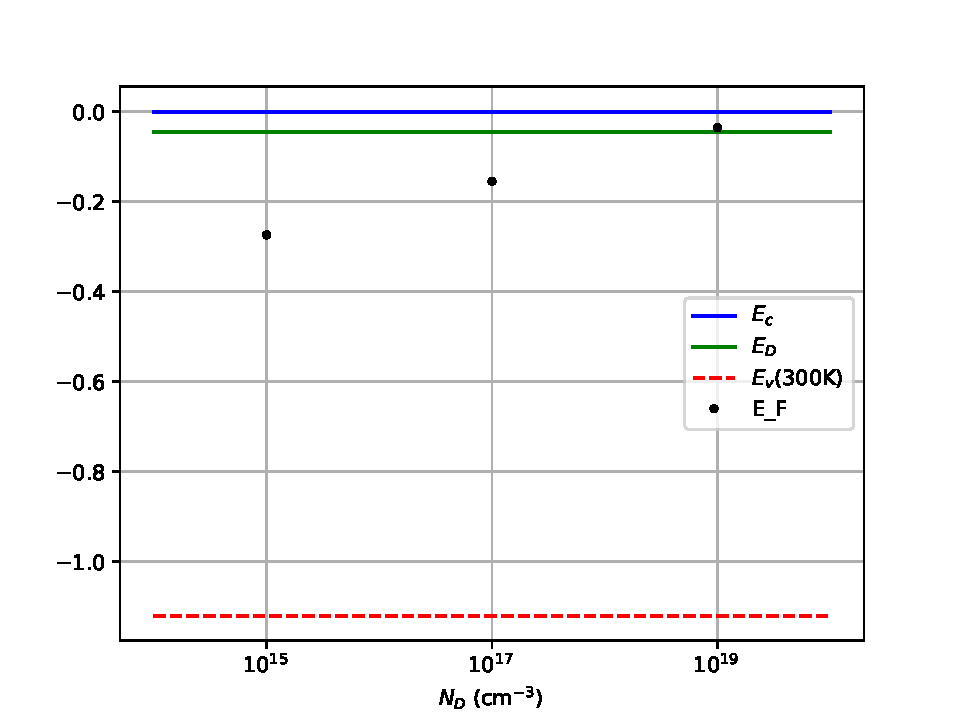
\includegraphics[width=0.9\linewidth]{Ejercicios/Ch_01/Ejercicio_01_8.pdf}
\end{center}



\begin{Enunciado}
\subsection*{Ejercicio 8}

Responde a las siguientes cuestiones:

\begin{enumerate}
	\item[a)] Utilizando la expresión para los átomos donadores ionizados dada en el ejercicio anterior, calcular la concentración de donadores sin ionizar para una muestra de silicio dopada con $10^{16}$ átomos/cm$^3$ de P ($E_D = 0.045$ eV) a una temperatura de 50 K. El nivel de Fermi está situado a 0.0459 eV por debajo de la banda de conducción.

	\item[b)] Una muestra de silicio a $T = 300$ K contiene una concentración de impurezas aceptoras $N_A = 10^{16}$ cm$^{-3}$. Determinar la concentración de átomos donantes que debe ser añadida para que el silicio sea tipo N y la energía de Fermi esté 0.25 eV por debajo del borde de la banda de conducción.
\end{enumerate}
\end{Enunciado}

\lipsum[1]



